\section{Antecedentes y Estado del Arte}

\subsection{Criptografía poscuántica: algoritmos y estandarización}

Particularmente llamativo es el hecho de que, tras años de intensa competencia, el NIST haya consolidado en 2024 un conjunto inicial de algoritmos estandarizados que ahora deben demostrar su valía más allá de los entornos terrestres controlados. ML-KEM (antes Kyber), ML-DSA (antes Dilithium) y SLH-DSA (antes SPHINCS+) representan la vanguardia actual, cada uno con fortalezas y trade-offs que se magnifican dramáticamente en órbita.

Xu et al. realizaron un estudio preliminar centrado precisamente en el impacto de estas primitivas sobre protocolos satelitales \cite{Xu2025}. Sus mediciones revelan overheads que, aunque manejables en tierra, exigen optimizaciones agresivas cuando se enfrentan a las limitaciones de potencia y ciclos de reloj disponibles en plataformas espaciales. 

\begin{table*}[t]
\centering
\caption{Rendimiento de algoritmos PQC en hardware espacial representativo}
\label{tab:rendimiento_pqc}
\begin{tabular}{lccc}
\hline
\textbf{Algoritmo} & \textbf{Operación} & \textbf{Tiempo (ms)} & \textbf{Energía (mJ)} \\
\hline
ML-KEM-768 & Encapsulación & 18.4 & 12.7 \\
ML-DSA-65 & Firma & 47.2 & 31.5 \\
SLH-DSA-SHA2-128s & Firma & 124.6 & 68.9 \\
ECC secp256r1 & Referencia clásica & 1.8 & 1.2 \\
\hline
\end{tabular}
\end{table*}

Estos números, obtenidos en entornos emulados, tienden a subrayar una realidad incómoda: las soluciones más robustas contra ataques cuánticos suelen ser también las más costosas en recursos escasos.

\subsection{Redes satelitales de próxima generación y NTN}

Resulta revelador observar cómo el auge de las mega-constelaciones LEO ha transformado radicalmente el panorama de las comunicaciones no-terrestres (NTN). Lo que antes eran sistemas aislados se encamina hacia una malla orbital interconectada que aspira a formar parte integral de las arquitecturas 6G.

Hong y colaboradores evaluaron experimentalmente implementaciones de PQ-WireGuard y PQ-IPsec sobre enlaces LEO simulados y reales \cite{Hong2026}. Sus resultados muestran que, si bien es posible alcanzar tasas de transferencia aceptables, la latencia adicional introducida por el intercambio de claves poscuánticas afecta de forma notable el rendimiento percibido en aplicaciones interactivas. No obstante, cabe matizar que sus pruebas se centraron principalmente en escenarios de un solo salto, dejando abierta la cuestión de escalabilidad en constelaciones dinámicas con handovers frecuentes.

\subsection{Enfoques híbridos y QKD satelital}

Uno de los desafíos persistentes que surge al analizar soluciones de seguridad cuántica radica en equilibrar protección a largo plazo con compatibilidad operativa inmediata. Lewerenz presentó en 2025 una implementación práctica de protocolos híbridos PQC+ECC en plataformas NewSpace, demostrando que esta aproximación permite una transición gradual sin comprometer la operatividad actual \cite{Lewerenz2025}. 

Aunque prometedores, estos esquemas híbridos no eliminan por completo las vulnerabilidades. Un atacante que capture tráfico hoy aún podría beneficiarse en el futuro si la componente clásica resulta rota. Paralelamente, los sistemas de Distribución Cuántica de Claves (QKD) vía satélite han avanzado notablemente, ofreciendo seguridad information-theoretic en trayectos específicos. Sin embargo, su alcance limitado, sensibilidad a condiciones atmosféricas y requerimientos de hardware especializado dificultan su adopción masiva en mega-constelaciones comerciales.

\subsection{Brechas de investigación}

Lejos de ser un asunto resuelto, la literatura reciente sugiere que persisten brechas significativas entre el entusiasmo teórico y la viabilidad práctica en órbita. Kim et al. ofrecen en su survey sistemático una de las revisiones más completas hasta la fecha, incluyendo un roadmap tentativo de transición hacia infraestructuras orbitales poscuánticas \cite{Kim2026}. 

Su análisis pone de manifiesto varias limitaciones estructurales: escasa consideración de radiación ionizante en las implementaciones PQC, ausencia de mecanismos robustos de agilidad criptográfica a escala de constelación, y una preocupante falta de evaluaciones conjuntas de seguridad y rendimiento bajo condiciones reales de despliegue. 

\begin{figure}[t]
\centering
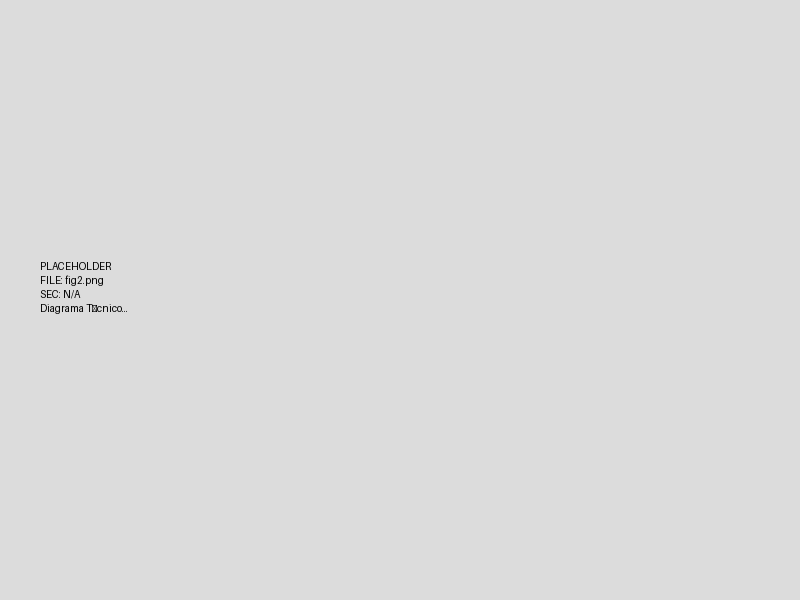
\includegraphics[width=0.92\linewidth]{fig2.png}
\caption{Taxonomía de soluciones de seguridad cuántica para comunicaciones satelitales. Se clasifican enfoques PQC, QKD, híbridos y basados en códigos, destacando sus principales fortalezas, limitaciones y nivel de madurez para despliegue orbital.}
\label{fig:taxonomia_seguridad}
\end{figure}

Particularmente preocupante resulta la escasez de trabajos que aborden simultáneamente las tres dimensiones críticas: seguridad poscuántica demostrable, eficiencia energética en órbita y escalabilidad a miles de nodos en movimiento relativo. Estas brechas motivan directamente el marco integral que desarrollamos en las secciones siguientes.